\subsection{Main Results}

\begin{table*}[t]
\centering
\caption{Main hotword retrieval results. Each cell reports F1 / R@1 (\%). Bold marks the best value among retrievers under the same training regime and benchmark.}
\label{tab:retrieval_main}
\small
\begin{tabular}{llcccc}
\toprule
Training & Method & AISHELL1-NE & ContextASR-ZH & ContextASR-EN & AISpeechMeeting \\
\midrule
ZH+EN & GLCLAP & 93.2 / 96.7 & 90.2 / 98.3 & 76.3 / 80.1 & 59.0 / 64.5 \\
ZH+EN & CLAR & 94.5 / 98.8 & 94.4 / \textbf{100.0} & 82.0 / 98.6 & 69.3 / 76.8 \\
ZH+EN & \textbf{TLDR} & \textbf{96.2} / \textbf{99.1} & \textbf{96.7} / \textbf{100.0} & \textbf{88.8} / \textbf{98.9} & \textbf{69.8} / \textbf{77.3} \\
\midrule
ZH-only & GLCLAP & 90.3 / 88.7 & 78.6 / 16.3 & 1.3 / 0.2 & 41.0 / 53.1 \\
ZH-only & CLAR & \textbf{96.9} / \textbf{99.5} & 80.6 / \textbf{96.7} & 1.3 / 1.4 & 49.3 / 54.5 \\
ZH-only & \textbf{TLDR} & 96.8 / 99.3 & \textbf{92.6} / 95.0 & \textbf{8.7} / \textbf{16.7} & \textbf{65.8} / \textbf{67.9} \\
\bottomrule
\end{tabular}
\end{table*}


Table~\ref{tab:retrieval_main} reports the main retrieval metrics. With ZH+EN training data, TLDR consistently improves F1 over GLCLAP and CLAR, with the largest gain on ContextASR-EN (+6.8 F1 over CLAR). Since R@5 and R@10 are nearly saturated on several benchmarks, F1 and R@1 provide the clearest main-paper comparison of candidate detection and top-ranked retrieval quality.

The advantage becomes more pronounced under the ZH-only setting. TLDR improves F1 by 12.0 points on ContextASR-ZH and 16.5 points on AISpeechMeeting over the strongest baseline, while matching CLAR on the cleaner AISHELL1-NE benchmark. This pattern suggests that token-level late interaction is especially useful when local hotword evidence is weak, noisy, or domain mismatched.

\begin{table*}[t]
\centering
\caption{Downstream contextual ASR results. Each cell reports hotword F1 / WER. Bold marks the best retrieval-based system; Oracle hotwords use ground-truth bias phrases and are reported only as an upper bound.}
\label{tab:decoding_main}
\small
\begin{tabular}{lcccc}
\toprule
Method & AISHELL1-NE & ContextASR-ZH & ContextASR-EN & AISpeechMeeting \\
\midrule
Raw & 92.6 / 1.75 & 92.1 / 2.59 & 77.4 / 10.97 & 23.3 / 18.90 \\
\textit{Oracle hotwords} & 99.8 / 0.51 & 99.3 / 1.35 & 99.4 / 4.56 & 97.1 / 9.58 \\
+GLCLAP & 98.3 / 0.77 & 99.0 / 1.40 & 95.4 / 5.73 & 67.5 / 14.86 \\
+CLAR & 98.5 / 0.88 & \textbf{99.2} / 1.36 & 95.4 / 5.61 & 77.3 / 12.79 \\
+\textbf{TLDR} & \textbf{98.7} / \textbf{0.71} & \textbf{99.2} / \textbf{1.34} & \textbf{97.3} / \textbf{5.03} & \textbf{80.3} / \textbf{12.40} \\
\bottomrule
\end{tabular}
\end{table*}


Table~\ref{tab:decoding_main} evaluates whether better retrieval translates into better contextual ASR. Compared with raw decoding, TLDR reduces WER by 59.4\%, 48.3\%, 54.1\%, and 34.4\% on AISHELL1-NE, ContextASR-ZH, ContextASR-EN, and AISpeechMeeting, respectively. Among retrieval-based systems, TLDR achieves the lowest WER on all benchmarks, showing that its retrieval gains are useful for downstream recognition rather than only improving standalone retrieval metrics.

\subsection{Secondary Metric Analysis}

\begin{figure*}[t]
  \centering
  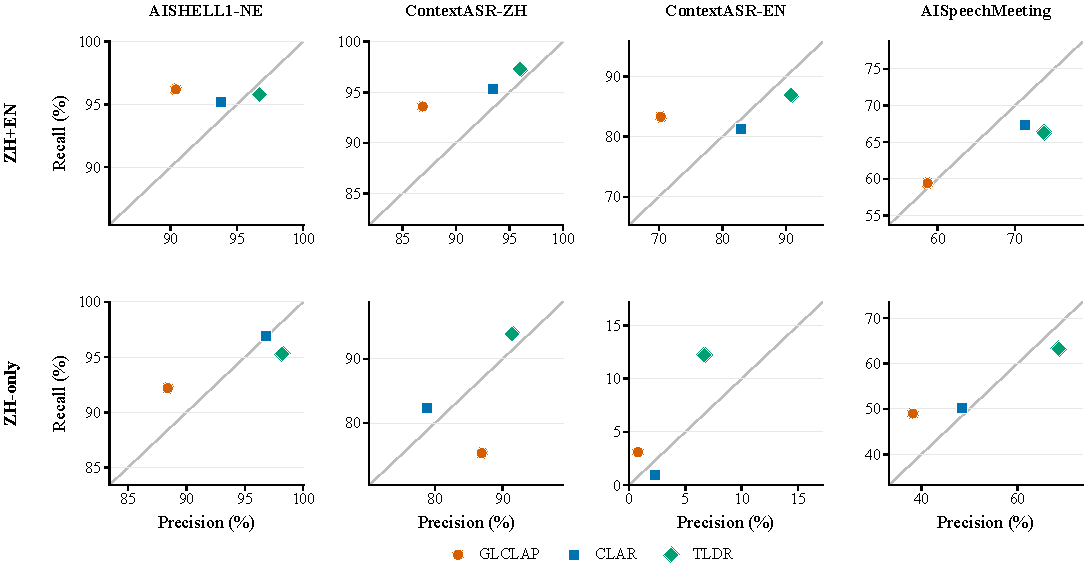
\includegraphics[width=0.98\textwidth]{figure/fig_retrieval_precision_recall.pdf}
  \caption{Precision-recall behavior of hotword retrieval systems. Each panel compares GLCLAP, CLAR, and TLDR on one benchmark under one training regime. TLDR generally shifts the operating point toward higher precision and recall, while CLAR remains competitive on the clean AISHELL1-NE setting. Axes are locally scaled for readability.}
  \label{fig:retrieval_pr}
\end{figure*}

\begin{figure*}[t]
  \centering
  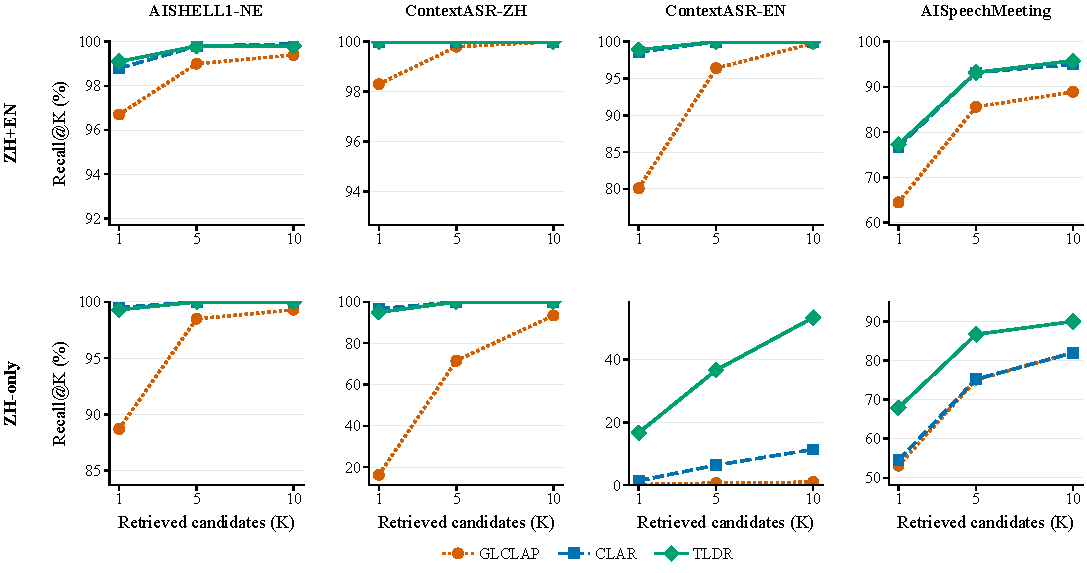
\includegraphics[width=0.98\textwidth]{figure/fig_retrieval_recall_at_k.pdf}
  \caption{Candidate ranking quality measured by Recall@K. While several ZH+EN results saturate at larger K, the ZH-only setting exposes larger differences: TLDR retains substantially higher ranked recall on ContextASR-EN and AISpeechMeeting. Axes are locally scaled for readability.}
  \label{fig:retrieval_ratk}
\end{figure*}

\begin{figure*}[t]
  \centering
  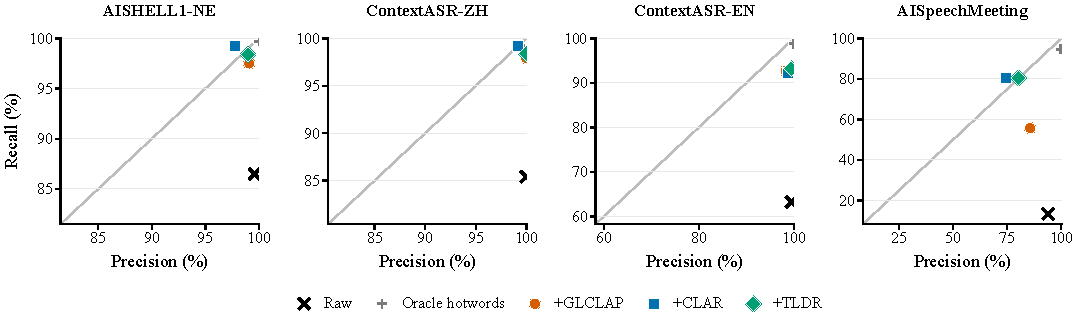
\includegraphics[width=0.98\textwidth]{figure/fig_decoding_precision_recall.pdf}
  \caption{Hotword precision-recall behavior after downstream decoding. Compared with retrieval baselines, TLDR produces a more balanced decoding operating point on the difficult English and meeting benchmarks, which is consistent with the WER reductions in Table~\ref{tab:decoding_main}. Axes are locally scaled for readability.}
  \label{fig:decoding_pr}
\end{figure*}

